\documentclass[a4paper]{scrreprt}

\usepackage{tikz}
\usetikzlibrary{positioning,calc}

\usepackage{lmodern}
\usepackage{microtype}
\usepackage[utf8]{inputenc}
\usepackage[T1]{fontenc}

\usepackage{amsmath}
\usepackage[retainorgcmds]{IEEEtrantools}

\usepackage{makeidx}

\title{Galois Theory}
\author{Wenda Zhou}

\begin{document}

\maketitle

\chapter{Introduction: cubics and quartics}

\paragraph{Quadratics}

\subparagraph{Case 1}
\begin{equation} \label{eq:case1}
X^2+b=0 \Rightarrow X=\pm \sqrt{-b}
\end{equation}

\subparagraph{Case 2}
\begin{equation} \label{eq:case2}
X^2-ax+b=0(x- \alpha)(x-\beta) = 0
\end{equation}
\begin{equation}
\text{where}
\begin{cases}
a &\!\!= \ \alpha + \beta \\
b &\!\!= \ \alpha\beta
\end{cases}
\end{equation}
we reduce this to \eqref{eq:case1}, i.e. $a=0$, put:
\begin{equation*}
\begin{cases}
\alpha{}' = \alpha - \frac{a}{2} \\
\beta{}'=\beta -\frac{a}{2}
\end{cases}
\end{equation*}
then we have that:
\begin{equation*}
\alpha + \beta = 0
\end{equation*}
\begin{IEEEeqnarray*}{rL}
\alpha{}'\beta{}' &= \alpha\beta -\frac{a}{2}(\alpha+\beta)+\frac{a^2}{4} \\
&=b-\frac{a^2}{2}+\frac{a^2}{4} \\
&=b-\frac{a^2}{4}
\end{IEEEeqnarray*}
hence $\alpha{}'$, $\beta{}'$ root of $X^2 + (b-\frac{a^2}{4})=0$, i.e. $\pm\sqrt{\frac{a^2}{4}-b}$ by \eqref{eq:case1}, thus we have that:
\begin{equation*}
\alpha, \beta = \frac{a}{2} \pm \sqrt{\frac{a^2}{4}-b}
\end{equation*}

\paragraph{Cubics}
\subparagraph{Case 3}
\begin{equation} \label{eq:case3}
X^3-c = 0 \Rightarrow X=\sqrt[3]{c}, \ \sqrt[3]{c}\zeta,\ \sqrt[3]{c}\zeta^2
\end{equation}
where $\zeta$ is the cubic root of unity, verifying:
\begin{equation*}
X^3-1=(X-1)(X^2+X+1) \Rightarrow \zeta, \ \zeta^2 = -\frac{1}{2} \pm \sqrt{-\frac{3}{4}} \quad \text{ by \eqref{eq:case2}}
\end{equation*}

\subparagraph{Case 4}
\begin{equation} \label{eq:case4}
X^3+bX-c=(X-\alpha)(X-\beta)(X-\gamma)=0
\end{equation}
where
\begin{equation*}
\begin{cases}
0=\alpha+\beta+\gamma \\
b=\alpha\beta+\beta\gamma+\gamma\alpha \\
c=\alpha\beta\gamma
\end{cases}
\end{equation*}
Reduce to case \eqref{eq:case2} and \eqref{eq:case3}, the Lagrange resolvents\index{Lagrange resolvent} of this cubic are defined as:
\begin{IEEEeqnarray*}{rClrCl}
x&=&\alpha+\beta\zeta+\gamma\zeta^2, \qquad &y &=&\alpha+\beta\zeta^2+\gamma\zeta \\
x\zeta&=&\alpha\zeta+\beta\zeta^2+\gamma, \qquad &y\zeta &=&\alpha+\beta+\gamma\zeta^2 \\
x\zeta^2&=&\alpha\zeta^2+\beta+\gamma\zeta, \qquad &y\zeta^2 &=&\alpha\zeta^2+\beta\zeta+\gamma \\
\end{IEEEeqnarray*}
hence we have that $x$, $x\zeta$, $x\zeta^2$ are roots of $X^3-x^3=0$ and $y$, $y\zeta$, $y\zeta^2$ are roots of $Y^3-y^3=0$.
Note that:
\begin{equation*}
\left\{
\begin{IEEEeqnarraybox}[][c]{rCl}
\IEEEstrut
\zeta^2+\zeta+1&=&0 \\
\alpha+\beta+\gamma&=&0
\IEEEstrut
\end{IEEEeqnarraybox}
\right.
\quad
\Rightarrow
\quad
\left\{
\begin{IEEEeqnarraybox}[][c]{rCl}
x+y&=&3\alpha \\
x\zeta^2+y\zeta&=&3\beta \\
x\zeta+y\zeta^2&=&3\gamma
\end{IEEEeqnarraybox}
\right.
\end{equation*}
hence, we have that:
\begin{equation*}
(\alpha, \beta, \gamma)=\left(\frac{x+y}{3}, \frac{x\zeta^2+y\zeta}{3}, \frac{x\zeta+y\zeta^2}{3}\right)
\end{equation*}
Note that:
\begin{IEEEeqnarray*}{rCl}
xy&=&\alpha^2+\beta^2+\gamma^2-\alpha\beta-\beta\gamma-\gamma\alpha \\
&=&(\alpha+\beta+\gamma)^2-3b \\
&=&-3b
\end{IEEEeqnarray*}
hence $x$, $y$ determine each other.
Now we also have that:
\begin{IEEEeqnarray*}{rCl}
x^3+y^3&=&(x+y)(x+y\zeta)(x+y\zeta^2) \\
&=&(x+y)(x+\zeta+y\zeta^2)(x\zeta^2+y\zeta) \\
&=&3\alpha\cdot{}3\beta\cdot{}3\gamma \\
&=&27c
\end{IEEEeqnarray*}
and also that $x^3y^3=-27b^3$, hence $x^3$, $y^3$ are the two roots of:
\begin{equation*}
X^2-27cX-27b^3=0
\end{equation*}
hence this is solved by \eqref{eq:case2}.

\subparagraph{Case 5}
\begin{equation} \label{eq:case5}
  X^3-aX^2+bX-c=(X-\alpha)(X-\beta)(X-\gamma) = 0
\end{equation}
We want to reduce this to \eqref{eq:case4}, by putting:
\begin{equation*}
  \alpha'=\alpha-\frac{a}{3}, \quad \beta'=\beta-frac{a}{3}, \quad \gamma'=\gamma-\frac{a}{3}
\end{equation*}
Then we have that $\alpha'+\beta'+\gamma'=0$, hence $\alpha'$, $\beta'$, $\gamma'$ are roots of:
\begin{equation*}
  X^3+\left(b-\frac{a^2}{3}\right)X-\left(\frac{2}{27}a^3-\frac{ab}{3}+c\right)=0
\end{equation*}
hence this is solved by \eqref{eq:case4}.

\paragraph{Quartics}

\subparagraph{Case 6}
\begin{equation} \label{eq:case6}
  X^4-aX^3+bX^2-cX+d=(X-\alpha)(X-\beta)(X-\gamma)(X-\delta)=0
\end{equation}
subtract $\frac{a}{4}$ from $\alpha$, $\beta$, $\gamma$, $\delta$ to reduce to case $a=0$. Now we reduce to \eqref{eq:case5}, by letting:
\begin{IEEEeqnarray*}{rCl?rCl?rCl}
  x&=&\alpha+\beta,& y&=&\alpha+\beta,& z &=& \alpha+\delta \\
  &=&-(\gamma+\delta)& &=&-(\beta+\delta) & &=& -(\beta+\gamma)
\end{IEEEeqnarray*}
since we assume that $a=\alpha+\beta+\gamma+\delta=0$. Hence we have that:
\begin{equation*}
  (\alpha, \beta, \gamma, \delta)=\left(\frac{x+y+z}{2}, \frac{x-y-z}{2}, \frac{-x+y-z}{2}, \frac{-x-y+z}{2}\right)
\end{equation*}
Note that we have:
\begin{IEEEeqnarray*}{rCl}
  xyz&=&(\alpha+\beta)(\alpha+\gamma)(\alpha+\delta) \\
  &=&\alpha^3+(\beta+\gamma+\delta)\alpha^2+(\beta\gamma+\gamma\delta+\delta\beta)\alpha+\beta\gamma\delta \\
  &=&c
\end{IEEEeqnarray*}
then we have that:
\begin{IEEEeqnarray*}{rCl}
  x^2&=&-(\alpha+\beta)(\gamma+\delta) \\
  y^2&=&-(\alpha+\gamma)(\beta+\delta) \\
  z^2&=&-(\alpha+\delta)(\beta+\gamma)
\end{IEEEeqnarray*}
thus note that we have that:
\begin{IEEEeqnarray*}{rCl}
  x^2+y^2+z^2&=&-2(\alpha\beta+\alpha\gamma+\alpha\delta+\beta\gamma+\beta\gamma+\gamma\delta) = -2b\\
  x^2y^2+y^2z^2+z^2x^2&=&b^2-4d\\
  x^2y^2z^2&=&c^2
\end{IEEEeqnarray*}
hence $x^2$, $y^2$, $z^2$ are the roots of:
\begin{equation*}
  X^3+2bX^2+(b^2-4d)X-C^2=0
\end{equation*}
this expression is the resolvent cubic\index{resolvent cubic} (of the quartic).

\paragraph{Summary}
We have the following symmetries:

\begin{tabular} { l c r }
  \eqref{eq:case1} & $\sqrt{-b}\longleftrightarrow{}-\sqrt{-b}$ & $\text{S}_2=\text{C}_2$ \\
  
  \eqref{eq:case1} $\Rightarrow$ \eqref{eq:case2} & rational (in field) & \\
  
  \eqref{eq:case3} & 
  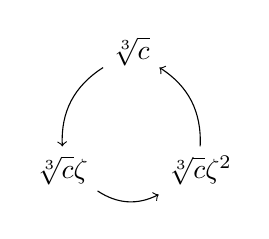
\begin{tikzpicture}[->]
    \node (1) {$\sqrt[3]{c}$};
    \node (2) at ($(1) + (-120: 1.75cm)$) {$\sqrt[3]{c}\zeta$};
    \node (3) at ($(1) + (-60: 1.75cm)$) {$\sqrt[3]{c}\zeta^2$};
    
    \path 
        (1) edge [bend right] node [left] {} (2)
        (2) edge [bend right] node [left] {} (3)
        (3) edge [bend right] node [left] {} (1);
  \end{tikzpicture} & $\text{A}_3=\text{C}_3$ \\
  
  \eqref{eq:case4} &
  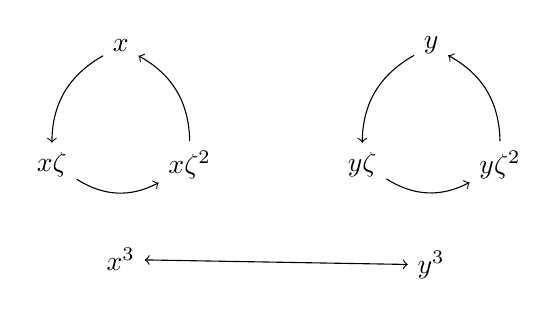
\begin{tikzpicture}[->] 
    \node (x1) {$x$};
    \node (x2) at ($(x1) + (-120: 1.75cm)$) {$x\zeta$};
    \node (x3) at ($(x1) + (-60: 1.75cm)$) {$x\zeta^2$};
    \node [right =3.5cm of x1](y1) {$y$};
    \node (y2) at ($(y1) + (-120: 1.75cm)$) {$y\zeta$};
    \node (y3) at ($(y1) + (-60: 1.75cm)$) {$y\zeta^2$};    
    
    \node [below = 2.25cm of x1](x) {$x^3$};
    \node [below = 2.25cm of y1](y) {$y^3$};

    \path 
        (x1) edge [bend right] node [left] {} (x2)
        (x2) edge [bend right] node [left] {} (x3)
        (x3) edge [bend right] node [left] {} (x1);
    \path 
        (y1) edge [bend right] node [left] {} (y2)
        (y2) edge [bend right] node [left] {} (y3)
        (y3) edge [bend right] node [left] {} (y1);
    \path[<->]
        (x) edge node {} (y);
  \end{tikzpicture} & \\
  \eqref{eq:case4} $\Rightarrow$ \eqref{eq:case5} & rational (in field) & \\
  
\end{tabular}
\end{document}
